\section{Illustrative Examples}\label{sec_example}


%We provide precise explanations to the phenomena of negative transfer in multi-task learning.
%We provide tight bounds on the bias and variance of the multi-task estimator for two tasks.
%The results in Section \ref{sec_general} show when multi-task learning outperforms single-task learning for general task covariance matrices and ground truth model parameters.
%In particular, the general conditions depend on specific properties of task data such as the covariate shift matrix.
%However, the conditions given by the limiting bias and variance of multi-task learning can be difficult to interpret.
%The goal of this section is to address this issue.
%We interpret the limiting bias and variance equations in an isotropic covariance setting that is described below and a simplified covariate-shifted setting.
%We show that three properties of task data affect the performance of multi-task learning as follows.
%(i) \textit{Task similarity}: We explain the phenomenon of negative transfer precisely as tasks become more different.
%(ii) \textit{Sample ratio}: We further explain a curious phenomenon where increasing the sample ratio between the source and target task helps initially, but hurts eventually.
%(iii) \textit{Covariate shift}: Finally, we show that as the sample size of the source task increases, we show that the covariate shift worsens the performance of the multi-task estimator.
%Finally, we provide a extend our results from two tasks to many tasks with the same features.
%We explain from three perspectives, including \textit{task similarity}, \textit{sample size} and \textit{covariate shift}.
%We show how negative transfer occurs by varying task similarity or sample size.
%Then we show that when source task sample size becomes large, covariate shift causes more negative effects.
We illustrate our main results, Theorem \ref{thm_many_tasks}, Theorem \ref{thm main RMT} and Corollary \ref{thm_main_informal}, in a simplified setting.
For this setting, we simulate several empirical phenomena that are well-known in hard parameter sharing approaches.
We use our results to explain the empirical phenomena.



%	The labels are $Y_i = X_i\beta_i + \varepsilon_i$, where $\e_i$ consists of i.i.d. entries with mean zero and variance $\sigma^2$.
%	For our purpose, it is enough to think of the order of $d$ being $1/\sqrt{p}$ and $pd^2/\sigma^2$ being constant.
%The more precise conditions on the relations between $d^2$, $\sigma^2$ and $\kappa^2$ are given in  \eqref{choiceofpara}.
%	We assume that all the random variables have subexponential decay, while keeping in mind that our results can be applied under weaker moments assumptions as shown in Appendix \ref{sec_maintools}.

%In the isotropic model, we show that as we increase the distance between $\beta_1$ and $\beta_2$ (or $d$), there is a transition from positive transfer to negative transfer in MTL.
%We measure model dissimilarity as $\norm{\beta_1 - \beta_2}^2$, which is the distance between source and target in the isotropic model.
%Figure \ref{fig_model_shift} provides a simulation when $p = 200$.
%{The rest of parameter settings can be found in Appendix \ref{app_synthetic}.}
%Our result below will provide an explanation to this phenomenon.
%Based on Theorem \ref{thm_model_shift}, we derive the transition threshold in the following proposition.
%We introduce the following notations.
%{\begin{align*}
%	\Psi(\beta_1, \beta_2) = {\ex{\bignorm{\beta_1 - \beta_2}^2}} / {\sigma^2},  \quad \Phi(\rho_1, \rho_2) = \frac{(\rho_1 + \rho_2 - 1)^2}{\rho_1 (\rho_1 + \rho_2) (\rho_2 - 1)}.
%\end{align*}}

\subsection{Sample Efficiency}

observed in Taskonomy \cite{ZSSGM18}.


\subsection{Sample Imbalance}

\noindent\textbf{Isotropic features and models.}
	Imagine that we have two tasks and the covariates of both tasks have isotropic covariance matrices.
%	Each task has sample size $n_1 = \rho_1 \cdot p$ and $n_2 = \rho_2 \cdot p$.
	%And $X_1\in\real^{n_1\times p}, X_2\in\real^{n_2\times p}$ denote the covariates of the two tasks, respectively.
	For the ground truth linear model, we consider a random-effects model where the two tasks differ by an independent Gaussian vector.
	Specially, for task two, we assume that its model parameter, denoted by $\beta_2$, consists of i.i.d. Gaussian entries with mean zero and variance $\kappa^2$.
	For task one, we assume that its model parameter, denoted by $\beta_1$, is equal to $\beta_2$ plus i.i.d. Gaussian entries with mean $0$ and variance $d^2$.
	Therefore, the two tasks have different ground truth models. In particular, the distance between $\beta_1$ and $\beta_2$ roughly scales as $d^2 \cdot p$.

\begin{example}[Varying model distance]
\end{example}

Using Theorem \ref{thm main RMT}, %our techniques described later in Section \ref{sec_general}, 
we derive the limiting prediction loss of the hard parameter sharing estimator.
Without loss of generality, we describe the result for task two and remark that a similar result for task one holds.

\begin{corollary}[Derived from Theorem \ref{thm main RMT}]
	Assume that the isotropic setting described above holds, and that there exists a small constant $c_0>0$ such that the signal-to-noise ratios satisfy that
\be\label{choiceofpara0}
p^{ c_0} \le \frac{p\kappa^2}{\sigma^2 }  \le p^{1-c_0},\quad  \frac{pd^2}{\sigma^2}=\OO(1).
\ee
	Let $B, W_1, W_2$ be the global minimum of equation \eqref{eq_mtl}. Then with high probability, the prediction loss of the hard parameter sharing estimator for task two satisfies:
	\begin{align*}
	 \left( 1-\frac{1}{\sqrt{\rho_1}}\right)^4 pd^2\cdot \frac{\rho_1^2 (\rho_1+\rho_2)}{(\rho_1 + \rho_2 - 1)^3} +\OO(p^{-c}\sigma^2)  \le L(\hat{\beta}_2^{\MTL}) -\frac{\sigma^2}{\rho_1+\rho_2-1} \\
	 \le  \left( 1+\frac{1}{\sqrt{\rho_1}}\right)^4 pd^2\cdot \frac{\rho_1^2 (\rho_1+\rho_2)}{(\rho_1 + \rho_2 - 1)^3} +\OO(p^{-c}\sigma^2 )
	 \end{align*}
	 for any constant $c\in (0,c_0)$.
	 \iffalse
	\begin{align*}
		& \bigabs{ L(\hat{\beta}_2^{\MTL}) - \frac{\sigma^2}{\rho_1 + \rho_2 - 1} - (1 + \frac{6}{\rho_1} + \frac{1}{\rho_1^2})pd^2\cdot \frac{\rho_1^2 (\rho_1+\rho_2)}{(\rho_1 + \rho_2 - 1)^3} } \\
		\le & 	\frac{4}{\sqrt{\rho_1}}(1 + \frac{1}{\rho_1})	pd^2\cdot \frac{\rho_1^2 (\rho_1+\rho_2)}{(\rho_1 + \rho_2 - 1)^3} + \oo(\sigma^2 + pd^2).
%	 \frac{\sigma^2}{\rho_1+\rho_2-1}+\left( 1-\frac{1}{\sqrt{\rho_1}}\right)^4  +\oo(\sigma^2 + pd^2)  \le \\
%	 \le  \frac{\sigma^2}{\rho_1+\rho_2-1}+\left( 1+\frac{1}{\sqrt{\rho_1}}\right)^4 pd^2\cdot \frac{\rho_1^2 (\rho_1+\rho_2)}{(\rho_1 + \rho_2 - 1)^3} +\oo(\sigma^2 + pd^2)
	 \end{align*}
	 \fi
\end{corollary}


It is well-known since the seminal work of Caruana \cite{C97} that how well multi-task learning performs depends on task relatedness.
We formalize this connection in the above isotropic setting, where we can perform explicit calculations.
We show that as we increase the distance between $\beta_1$ and $\beta_2$, there is a transition from positive transfer to negative transfer in MTL.
In particular, the bias of MTL increases as the distance between $\beta_1$ and $\beta_2$ increases.
Therefore, while the variance of MTL still reduces compared to STL, if the bias increases more than the amount of variance reduced, we will observe negative transfer.



\begin{proposition}[Task model distance]\label{prop_dist_transition}
	In the isotropic model, suppose that $\rho_1$ and $\rho_2 > 1$.
	Then
	%Whether $\te(\hat{\beta}_t^{\MTL})$ is lower than $\te(\hat{\beta}_t^{\STL})$ is determined by the ratio between $\Psi(\beta_1, \beta_2)$ and $\Phi(\rho_1, \rho_2)$:
	\begin{itemize}
		\item \textbf{Positive transfer:} If $\Psi(\beta_1, \beta_2) < \frac{1}{\nu} \cdot  \Phi(\rho_1, \rho_2)$, then w.h.p. over the randomness of $X_1,X_2$,
			\[ \te(\hat{\beta}_2^{\MTL}) < \te(\hat{\beta}_2^{\STL}). \]
		\item \textbf{Negative transfer:} If $\Psi(\beta_1, \beta_2) > {\nu} \cdot  \Phi(\rho_1, \rho_2)$, then w.h.p. over the randomness of $X_1,X_2$,
			$$\te(\hat{\beta}_2^{\MTL}) > \te(\hat{\beta}_2^{\STL}).$$
	\end{itemize}
	Here {\small$\nu = (1+\oo(1)) \cdot (1 - 1/\sqrt{\rho_1})^{-4}$}.
	Concretely, if $\rho_1 > 40$, then $\nu\in (1,2)$.
\end{proposition}


Proposition \ref{prop_dist_transition} simplifies Theorem \ref{thm_main_informal} in the isotropic model, allowing for a more explicit statement of the bias-variance tradeoff.
Concretely, $\Psi(\beta_1, \beta)$ and $\Phi(\rho_1, \rho_2)$ corresponds to $\Delta_{\bias}$ and $\Delta_{\vari}$, respectively.
%Roughly speaking, the transition threshold scales as $\frac{pd^2}{\sigma^2} - \frac{1}{\rho_1} - \frac{1}{\rho_2}$.
We apply Proposition \ref{prop_dist_transition} to the parameter setting of Figure \ref{fig_model_shift} (the details are left to Appendix \ref{app_synthetic}).
We can see that our result is able to predict positive or negative transfer  accurately and matches the empirical curve.
There are several unexplained observations near the transition threshold $0$, which are caused by the concentration error $\nu$.
%We fix the target task and vary the source task, in particular the parameter $d$ which determines $\norm{\beta_1 - \beta_2}$.
%Figure \ref{fig_model_shift} shows the result.
%We observe that Proposition \ref{prop_dist_transition} explains most of the observations in Figure \ref{fig_model_shift}.
The proof of Proposition \ref{prop_dist_transition} involves two parts.
First, in equation \eqref{eq_te_var}, the positive variance reduction effect scales with $n_1 = \rho_1 p$, the number of source task data points.
Second, we show that the negative effect of model-shift bias scales with $pd^2$, which is the expectation of $\norm{\beta_1 - \beta_2}^2$.
The proof of Proposition \ref{prop_dist_transition} can be found in Appendix \ref{app_proof_31}.
A key part of the analysis shows that $\hat{W}_1 / \hat{W}_2$ is roughly equal to one in the isotropic model,
thus simplifying the general condition in Theorem \ref{thm_main_informal}.

\begin{figure}[!t]
	\begin{subfigure}[b]{0.32\textwidth}
		\centering
		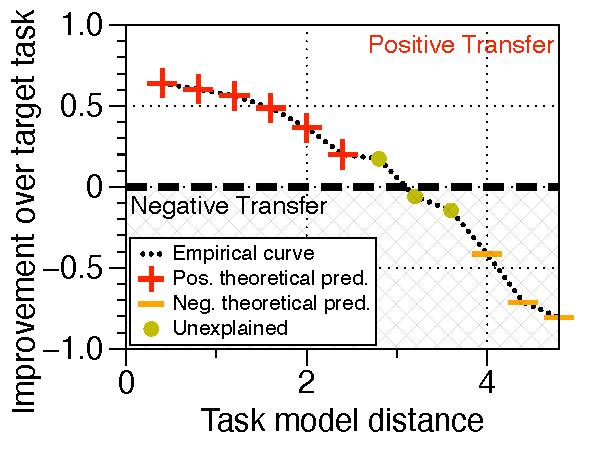
\includegraphics[width=0.98\textwidth]{figures/model_shift_phase_transition.pdf}
		\caption{Task similarity}
		\label{fig_model_shift}
	\end{subfigure}\hfill
	\begin{subfigure}[b]{0.32\textwidth}
		\centering
		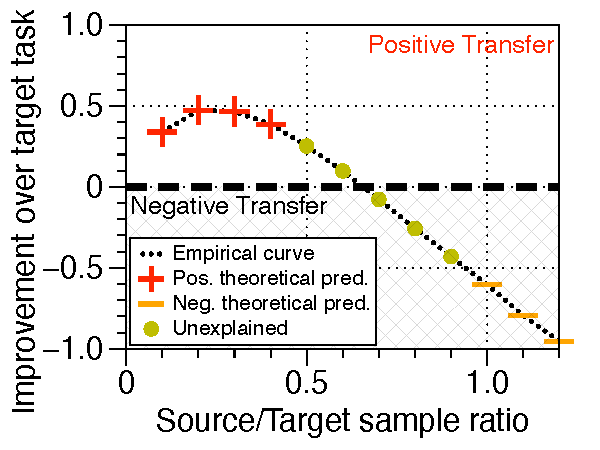
\includegraphics[width=0.98\textwidth]{figures/datapoints_phase_transition.pdf}
		\caption{Sample size}
		\label{fig_size}
	\end{subfigure}\hfill
	\begin{subfigure}[b]{0.32\textwidth}
		\centering
		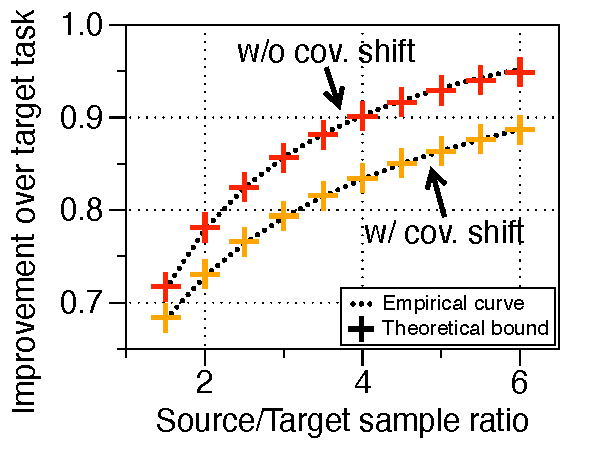
\includegraphics[width=0.98\textwidth]{figures/complementary.pdf}
		\caption{Covariate shift}
		\label{fig_covariate}
	\end{subfigure}
	\caption{%Three takeaways of our theory in Section \ref{sec_insight}.
	We observe a transition from positive to negative transfer as (a) \textit{task model distance} increases and (b) source/target \textit{sample ratio} increases.
	For the special case of having the same task model, we observe in (c) that as source/target \textit{sample ratio} increases, having \textit{covariate shift} worsens the performance of MTL.
	The $y$-axis measures the loss of STL minus MTL.}
	\label{fig_model_shift_phasetrans}
\end{figure}

%\subsection{Sample Ratio}\label{sec_data_size}

In classical Rademacher or VC based theory of multi-task learning, the generalization bounds are usually presented for settings where the sample sizes are equal for all tasks \cite{B00,M06,MPR16}.
%More generally, such results are still applicable when all task data are being added simultaneously.
On the other hand, uneven sample sizes between different tasks (or even dominating tasks) have been empirically observed as a cause of negative transfer \cite{YKGLHF20}.
For such settings, we have also observed that adding more labeled data from one task does not always help.
%On the other hand, we have observed that adding more labeled data does not always improve performance in multi-task learning.
In the isotropic model, we consider what happens if we vary the source task sample size.
Our theory accurately predicts a curious phenomenon, where increasing the sample size of the source task results in negative transfer!
Figure \ref{fig_size} provides a simulation result for such a setting.
We observe that as $n_1 / n_2$ increases, there is a transition from positive to negative transfer.

\begin{proposition}[Source/target sample ratio]\label{prop_data_size}
	In the isotropic model, suppose that $\rho_1 > 40$ and $\rho_2 > 110$ are fixed constants, and $\Psi(\beta_1, \beta_2) > 2/(\rho_2 - 1)$.
	Then we have that
	\begin{itemize}
		\item \textbf{Positive transfer:} If $\frac{n_1}{n_2} = \frac{\rho_1}{\rho_2} < \frac{1}{\nu} \cdot \frac{1 - 2\rho_2^{-1}}{\Psi(\beta_1, \beta_2) (\rho_2 - 1) - \nu^{-1}}$, then w.h.p. $$\te(\hat{\beta}_2^{\MTL}) < \te(\hat{\beta}_2^{\STL}).$$
		\item \textbf{Negative transfer:} If $\frac{n_1}{n_2} = \frac{\rho_1}{\rho_2} > {\nu} \cdot \frac{1 - 2\rho_2^{-1}}{\Psi(\beta_1, \beta_2) (\rho_2 - 3/2) - \nu}$, then w.h.p. $$\te(\hat{\beta}_2^{\MTL}) > \te(\hat{\beta}_2^{\STL}).$$
	\end{itemize}
\end{proposition}
Proposition \ref{prop_data_size} describes the bias-variance tradeoff in terms of the sample ratio $\rho_1 / \rho_2$.
We apply the result to the setting of Figure \ref{fig_size} (described in Appendix \ref{app_synthetic}).
There are several unexplained observations near $y = 0$ caused by $\nu$.
The proof of Proposition \ref{prop_data_size} can be found in Appendix \ref{app_proof_32}.

\subsection{Covariate Shift} \label{sec_covshift}
So far we have considered the isotropic model where $\Sigma_1 = \Sigma_2$.
This setting is relevant for settings where different tasks share the same input features such as multi-class image classification.
In general, the covariance matrices of the two tasks may be different such as in text classification.
In this part, we consider what happens when $\Sigma_1 \neq \Sigma_2$.
We show that when $n_1 / n_2$ is large, MTL with covariate shift can be suboptimal compared to MTL without covariate shift.

\noindent\textit{Example.}
	We measure covariate shift by $M = \Sigma_1^{1/2} \Sigma_2^{-1/2}$ similar to Theorem \ref{thm_main_informal}.
	We assume that the two tasks have the same ground truth model parameters, that is, $\beta_1 = \beta_2$ and $\Psi(\beta_1, \beta_2) = 0$.
	We compare two cases: (i) when $M = \id_{p\times p}$; (ii) when $M$ has $p/2$ singular values that are equal to $\lambda$ and $p/2$ singular values that are equal to $1 / \lambda$.
	Hence, $\lambda$ measures the severity of the covariate shift.
	Figure \ref{fig_covariate} shows a simulation of this setting by varying $\lambda$.
	We observe that as source/target sample ratio increases, the performance gap between the two cases increases.

%By applying Lemma \ref{lem_cov_shift_informal}, we find that when $n_1 / n_2$ is large, having no covariate shift is the optimal choice provided that the determinant of $M^{\top}M$ is bounded.
We compare different choices of $M$ that belong to the following bounded set.
Let $\lambda_i$ be the $i$-th singular value of $M$.
Let $\mu_{\min} < \mu < \mu_{\max}$ be fixed values that do not grow with $p$.
{\begin{align*}
		\cS_{\mu}\define\bigset{M \left| \prod_{i=1}^p \lambda_i \le \mu^p, \mu_{\min} \le \lambda_i\le \mu_{\max}, \text{ for all } 1\le i\le p\right.},
\end{align*}}
%	We assume that $\beta_1$ and $\beta_2$ are generated following the isotropic model with $d = 0$.
\begin{proposition}[Covariate shift]\label{prop_covariate}
	For the setting of the example above, assume that $\beta_1 = \beta_2$, $\rho_1$ and $\rho_2$ are both greater than one.
	Let $g(M)$ denote the prediction loss of $\hat{\beta}_t^{\MTL}$ when $M = \Sigma_1^{1/2}\Sigma_2^{-1/2} \in\cS_{\mu}$.
	We have that
		\[ g(\mu\id) \le \bigbrace{1+ \bigo{{\rho_2}/{\rho_1}  }} \min_{M\in\cS_{\mu}} g(M). \]
\end{proposition}


\iffalse

 \begin{claim}\label{claim_covar_shift}
		In the setting of Proposition \ref{prop_covariate}, for any $M\in \cal S_\mu$ we have that
		\[ g(M)=(1+\OO(p^{-\e}))\cdot \sigma^2  \bigtr{\Sigma_2(X_1^{\top}X_1  + X_2^{\top}X_2)^{-1} }  \quad \text{w.h.p.} \]
	\end{claim}

%Finally, in this subsection we prove Proposition \ref{prop_covariate}, which shows that $\te(\hat{\beta}_2^{\MTL})$ is minimized approximately when $M$ is a scalar matrix, provided that there is enough source data.

\begin{proof}[Proof of Proposition \ref{prop_covariate}]
 

 
 Denote the minimizer of $g$ by 
$$M_0:=\argmin_{M\in \cal S_{\mu}}g(M).$$ 
We now calculate $g(M_0)$. 


Now using Lemma \ref{lem_cov_shift}, we obtain that with high probability,
\begin{align}\label{gvar_extra}
g(M_0)= \frac{\sigma^2}{\rho_1+\rho_2}\cdot \frac1p\tr\left( \frac{1}{a_1(M_0)\cdot M_0^\top M_0 + a_2(M_0)}\right) \cdot \left(1 +\OO(p^{-\e})\right).
\end{align}
From equation \eqref{eq_a12extra}, it is easy to obtain the following estimates on $ a_1(M)$ and $a_2(M)$ for any $M\in \cal S_\mu$:
\be\label{est_a12extra}
\frac{\rho_1-1}{\rho_1+\rho_2} < a_1(M)<  \frac{\rho_1+\rho_2-1}{\rho_1+\rho_2},\quad a_2(M) < \frac{\rho_2}{\rho_1+\rho_2}.
\ee
Inserting \eqref{est_a12extra} into \eqref{gvar_extra} and using $ M_0^\top M_0\succeq \mu_{\min}^2$, we obtain that with high probability,
\begin{align}\label{approximateteM}
\left(1+\frac{\rho_2}{(\rho_1-1)\mu_{\min}^2}\right)^{-1}h(M_0) \cdot \left(1 - \OO(p^{-\e})\right) \le g(M_0) \le h(M_0) \cdot \left(1 +\OO(p^{-\e})\right),
\end{align}
where
$$h(M_0):=\frac{\sigma^2}{(\rho_1+\rho_2)a_1(M_0)}\cdot \frac1p\tr\left( \frac{1}{M_0^\top M_0}\right) .$$
%With these two bounds, we can easily conclude \eqref{approxteM}. 
%
%We have that the test error satisfies
%\be\label{approxteM}  te(M)\left(1 -  \frac{n_2}{n_1-p} \frac{1}{\lambda_p^2 + \frac{n_2}{n_1-p}}\right)  \le  \frac{\sigma^2}{n_1+n_2}\tr\left( \frac{1}{a_1M^\top M + a_2}\right) \le te(M),\ee
%where $\lambda_p$ is the smallest singular value of $p$ and
%$$te(M):= \frac{\sigma^2}{a_1(n_1+n_2)}\tr\left( \frac{1}{M^\top M}\right) .$$
%Moreover, for all $M$ satisfying \eqref{GMcons}, the minimum of $te(M)$ is attained when $M= a\id$.
By AM-GM inequality, we observe that 
$$\tr\left( \frac{1}{M^\top M}\right) = \sum_{i=1}^p\frac{1}{\lambda_i^2}$$
is minimized when $\lambda_1 = \cdots\lambda_p=\mu$ under the restriction $\prod_{i=1}^p\lambda_i\le \mu^p$. Hence we get that 
\be\label{AMGM} h(M_0) \le \frac{\sigma^2}{\mu^2 (\rho_1+\rho_2)a_1(M_0)}.\ee
On the other hand, when $M=\mu \id$, applying Lemma \ref{lem_cov_shift} we obtain that with high probability,
\begin{align}\label{gvar_extra2}
\begin{split}
g(\mu \id)&= \frac{\sigma^2}{\rho_1+\rho_2}\cdot \frac1p\tr\left( \frac{1}{\mu^2 a_1 (\mu\id) + a_2(\mu\id)}\right) \cdot \left(1 +\OO(p^{-\e})\right)\\
&\le \frac{\sigma^2}{\mu^2(\rho_1+\rho_2)a_1 (\mu\id)}.
\end{split}
\end{align}
Combining \eqref{est_a12extra}, \eqref{approximateteM}, \eqref{AMGM} and \eqref{gvar_extra2}, we conclude the proof.
%, we conclude that the sum $\sum_{i=1}^p\lambda_i^{-1}$ is smallest when $\lambda_1=\cdots=\lambda_p = a$.
\end{proof}
\fi

Proposition \ref{prop_covariate} shows that when the sample ratio is large, having no covariate shift gives the optimal performance for multi-task learning.
The proof of Proposition \ref{prop_covariate} can be found in Appendix \ref{app_proof_33}.
%Proposition \ref{prop_covariate} implies that when $\rho_1\gg \rho_2$, having no covariate shift is the optimal choice for choosing the source task.
%This provides evidence that covariate shift is unfavorable when there are many source task datapoints,

%\todo{} To complement the result, we show an example when the statement is not true if $n_1 \le n_2$.

%We ask: is it better to have $M$ as being close to identity, or should $M$ involve varying levels of singular values?
%Understanding this question has implications for applying normalization methods in multi-task learning \cite{LV19,CBLR18,YKGLHF20}.
%We show that if $n_1$ is much larger than $n_2$, then the optimal $M$ matrix should be proportional to identity, under certain assumptions on its range of singular values (to be formulated in Proposition \ref{prop_covariate}).
%On the other hand, if $n_1$ is comparable or even smaller than $n_2$, we show an example where having ``complementary'' covariance matrices is better performing than having the same covariance matrices.




